\begin{frame}{The Need for Decentralization}
    \begin{columns}[T] % align columns
        \begin{column}{.48\textwidth}
            \begin{figure}
                \centering
                \includegraphics[height = .7\textheight]{figures/bad_messages_enzo}
            \end{figure}
        \end{column}%
        \hfill%
        \begin{column}{.48\textwidth}
            \bigskip
            \begin{itemize}
                \item Data is stored in silos
                \item Reduces interoperability
                \item Stifles innovation
            \end{itemize}
        \end{column}%
    \end{columns}
    \note{
    \begin{itemize}
    \item How many different chat applications do you use?
    \item Why is data centralized by the companies, instead of you controlling it and giving it to others
    \item We should be able to chat with any application to every other application
    \end{itemize}
    }
\end{frame}

\begin{frame}{Decentralized Environments}
    \begin{columns}[T] % align columns
        \begin{column}{.48\textwidth}
        
            \begin{figure}
                \centering
                \includegraphics[height = .7\textheight]{figures/decentralizedMessageStorage}
            \end{figure}
        
        \end{column}%
        \hfill%
        \begin{column}{.48\textwidth}
            \bigskip
            \begin{itemize}
                \item Data is stored in personal data vaults
                \item Applications can request usage of the data
                \item Facilitates interoperability \& innovation
            \end{itemize}
        \end{column}%
    \end{columns}
\end{frame}


\begin{frame}{Querying Decentralized Environments}
    \begin{columns}[T] % align columns
        \begin{column}{.48\textwidth}
            \begin{figure}
                \centering
                \includegraphics[height = .80\textheight]{figures/ManySourceHowToFindNoText}
            \end{figure}
        \end{column}%
        \hfill%
        \begin{column}{.48\textwidth}
            \bigskip
            \begin{itemize}
                \item How do we find decentralized sources?
                \item How do we query decentralized sources?
            \end{itemize}
        \end{column}%
    \end{columns}
    \note{
    Explain challenges with decentralized environments:
    \begin{itemize}
    \item Finding the relevant data to query over (where can we dereference the data vaults)
    \item How do we issue queries over such decentralized vaults
    \item How do we \emph{efficiently} query these sources?
    \end{itemize}
    }
\end{frame}

\begin{frame}{Link Traversal-based Query Processing}
    \begin{columns}[T] % align columns
        \begin{column}{.48\textwidth}
        
            \begin{figure}
                \centering
                \includegraphics[height = .80\textheight]{figures/queryWithLinkTraversal1}
            \end{figure}
        
        \end{column}%
        \hfill%
        \begin{column}{.48\textwidth}

            \begin{figure}
                \centering
                \includegraphics[height = .63\textwidth]{figures/queryImage}
            \end{figure}

        \end{column}%
    \end{columns}
\end{frame}

\begin{frame}{Link Traversal-based Query Processing}
    \begin{columns}[T] % align columns
        \begin{column}{.48\textwidth}            
            \begin{figure}
                \centering
                \includegraphics[height = .80\textheight]{figures/queryWithLinkTraversal2}
            \end{figure}            
        \end{column}%
        \hfill%
        \begin{column}{.48\textwidth}
            \bigskip
            \begin{itemize}
                \item Start with seed documents
                \item Follow links discovered in previously dereferenced documents
            \end{itemize}
        \end{column}%
    \end{columns} 
\end{frame}

\begin{frame}{Link Traversal-based Query Processing}
    \begin{columns}[T] % align columns
        \begin{column}{.48\textwidth} 
            \begin{figure}
                \centering
                \includegraphics[height = .80\textheight]{figures/queryWithLinkTraversal3}
            \end{figure}
        \end{column}%
        \hfill%
        \begin{column}{.48\textwidth}
            \bigskip
            \begin{itemize}
                \item Terminate when all links are followed
                \item Stream query results from data discovered
            \end{itemize}
        \end{column}%
    \end{columns}
\end{frame}

\begin{frame}{Finding Data Within Personal Data Vaults}
    \begin{columns}[T] % align columns
        \begin{column}{.48\textwidth}          
            \begin{figure}
                \centering
                \includegraphics[height = .80\textheight]{figures/interiorOfDataVault}
            \end{figure}
        \end{column}%
        \hfill%
        \begin{column}{.48\textwidth}
            \bigskip
            \begin{itemize}
                \item Data vaults can have a file-like structure 
                \item Parts of this file 'tree' can be irrelevant for a given query
                \item Identifying this is vital for performance.
            \end{itemize}
        \end{column}%
    \end{columns}
    \note{
    \begin{itemize}
    \item Within data vaults there exists a file-like directory structure we can use link traversal for
    \item Part of this vault might be irrelevant for a given query, like all posts not on the topic of semantic web
    \item We need to identify this 
    \end{itemize}
    }
\end{frame}

\begin{frame}{Strenghts \& Weaknesses}
    \begin{columns}[T] % align columns
        \begin{column}{.48\textwidth}
            \color{green}Pros:
            \begin{itemize}
                \item Iterative discovery of new sources
                \item Designed to query large decentralized environments
            \end{itemize}
        \end{column}%
        \hfill%
        \begin{column}{.48\textwidth}
        \end{column}%
    \end{columns}
    \note{
    Here we primarily introduce the need for extensive optimization due to difficulties in query optimization
    }
\end{frame}

\begin{frame}{Strenghts \& Weaknesses}
    \begin{columns}[T] % align columns
        \begin{column}{.48\textwidth}
            \color{green}Pros:
            \begin{itemize}
                \item Iterative discovery of new sources
                \item Designed to query large decentralized environments
            \end{itemize}
        \end{column}%
    \hfill%
        \begin{column}{.48\textwidth}
            \color{red}Cons:
            \begin{itemize}
                \item Lack of prior knowledge of the data makes query optimization difficult
            \end{itemize}
        \end{column}%
    \end{columns}
\note{
Here, we primarily introduce the need for extensive optimization due to difficulties in query optimization
}
\end{frame}



% Flowchart for hypothesis
% Callback to the different avenues for optimization (link prio / query plan)
% Explain query plan
% Figure that explains the difference between state-of-the-art and LTQP, especially since we don't know the queried data
% while relational / SPARQL knows all data we query and can use that
% More details on what query usage patterns we want to investigate
% Grammarly!!

